% !TeX root = ../thuthesis-example.tex

\chapter{引言}


\section{研究背景}\label{1-background}


物联网(IoT)的概念最初于1999年提出,通常指使用网络连接多种信息感知设备,实现信息交换,从而让系统能够自动的、实时的对物体进行识别、定位、追踪、监控并触发相应事件。\cite{王保云2009物联网技术研究综述木}。目前,应用物联网的领域包括智能家居、可穿戴设备、工业物联网、智慧医疗、智慧城市、智慧农业等。根据相关研究,2025年全球GDP的4\% - 11\%是由物联网贡献\cite{mouha2021internet}。

工业物联网(Industrial Internet of Things, IIoT)\cite{sisinni2018industrial}是物联网的一个细分领域,通过在工业领域部署传感器、仪器、设备和其他物联网装置,通过数据采集、传输、分析处理、应用而完成工业流程、实现效率提升,完成新型商业模式的构建,推动传统工业向数字化、智能化的转型升级,在智能制造、能源领域、物流运输、医疗保健、农业领域等都有着广泛的应用。

在工业物联网中,时间序列数据(Time-Series Data)\cite{dunning2015tsdb}扮演着至关重要的角色。在时序数据中,每个数据点都与一个特定的时间戳相关联,表明该数据是在何时被记录或观测到的,工业环境中部署的各种传感器、仪器和设备会持续不断地产生大量的时序数据。时序数据具备以下的这些特点:

1. 产生速度快。工业设备上的各种传感器,如温度传感器、振动传感器、压力传感器等,可能每秒甚至每毫秒产生多个数据点,监测设备的运行状态。一条生产线上可能部署成百上千个传感器,瞬间产生大量数据。国际风电标准 IEC 61400-25 规定,一台风机每秒需
要采集 225KB 的工业数据,在某些极端工况下数据的采集频率需要提升至 8 KHz\cite{PZKX202005001}。

2. 总量巨大。时序数据以较高的频率持续产生,并且往往需要长期保存以进行历史分析、趋势预测等,因此其累积的总量往往非常庞大。长安汽车集团的车联网为每一辆生产的汽车部署了数千个传感器,每年产生的原始数据量超过13PB。

3. 种类丰富。不同的行业和应用领域关注不同的指标和数据类型,例如工业领域的设备运行参数,金融领域的交易价格和成交量,医疗领域的生理指标,环境监测领域的污染物浓度等。时序数据可以包括数值型数据(例如温度、压力、速度)、布尔型数据(例如设备状态:开/关)、离散型数据(例如故障代码)甚至文本型数据(例如日志信息)等。

时序数据库\cite{naqvi2017timeseriesdb}是针对时序场景优化的数据管理系统。相较于关系性数据库\cite{codd2007relational}和NoSQL数据库\cite{han2011surveynosql},时序数据库通常具备更低的写入延迟和更高的写入吞吐、更强的存储压缩能力、高效的时间范围查询和聚合等。在实现上,时序数据库通常采用LSM\cite{o1996lsmtree}引擎进行数据存储,内置了丰富的基于时间窗口的聚合查询函数、专门的压缩算法等。
常见的时序数据库包含Apache IoTDB\cite{wang2020iotdb}、InfluxDB\cite{shahid2019influxdb}、TDEngine\cite{tdengine_website}、DolphinDB\cite{dolphindb_website}、OpenTSDB\cite{opentsdb_website}、TimescaleDB\cite{timescale_website}等。

Apache IoTDB是一个开源的分布式时序数据库,目前是Apache基金会的顶级项目,具有为时间序列数据所优化的存储引擎、查询引擎以及分布式框架,可以满足工业物联网领域对海量时间序列数据高速写入、存储、快速读取以及复杂查询的需求,凭借着高性能、高可用性等在工业物联网、智能城市、智能电网等领域得到了广泛应用。

分布式数据库中的高可用性和容错性\cite{gray2002high}对于确保业务连续性至关重要。系统故障和服务中断会导致直接的经济损失、损害企业的声誉、甚至在医疗交通等关键领域引发严重的安全风险。
分布式数据库实现高可用的关键在于消除单点故障,进行数据和服务的冗余,并在冗余节点之间可靠地进行故障转移,从而应对多种不同类型的故障,包括节点故障、网络分区和软件错误等。

在高可用性的建设中,数据复制\cite{milani2017systematic}是关键策略。通过在多个节点上存储数据的副本,从而保证即使单一或多个节点发生故障,数据依然可以从其他节点获取。共识协议对于维护多个数据副本的一致性至关重要,共识协议保证了系统在暂时性错误的情况下,所有数据副本最终能够达成一致的状态。系统可以通过自动检测故障,并在发现故障之后进行自动错误恢复(Failover)\cite{mohammed2017failover},将请求重定向健康的副本上,从而减少故障时的停止服务时间。


恢复时间目标 (Recovery Time Objective, RTO) 和恢复点目标 (Recovery Point Objective, RPO) 是衡量高可用性的两个重要指标。RTO 是指从服务中断到恢复服务所需的最长可接受时间,而 RPO 是指在发生中断后可能丢失数据的最大可接受时间。这些指标有助于组织设定明确的恢复目标,并评估其高可用性解决方案的有效性。


\section{研究动机}\label{1-motivation}

在Apache IoTDB分布式架构设计之初,高可用性和容错能力就被定为重要的目标之一。
高可用性是保障工业物联网相关应用稳定的基石,IoTDB的设计必须确保系统能够在各种情况下持续提供服务,最大限度地减少停机时间,保证数据的连续写入和读取,从而满足工业场景对实时性和可靠性的要求。
容错能力是IoTDB内部应对系统复杂性和潜在故障的关键。分布式系统由多个节点组成,单个节点的故障是不可避免的。在工业物联网环境中,设备种类繁多,网络环境复杂,更容易出现硬件故障、网络中断等问题。IoTDB 的设计需要具备强大的容错机制,即使部分节点发生故障,系统也能够自动地检测到并进行恢复,保证数据的完整性和服务的连续性。


在本文的工作之前,Apache IoTDB围绕高可用性和容错能力已经做了大量的建设,包含但不限于:

1. IoTDB建立了统一的共识协议统一框架,为数据维护了多个副本,避免了因单点故障产生的数据丢失的问题。
通过一致的框架建设,IoTDB还实现了性能和一致性级别不同的各类共识协议,包括基于强一致性协议的RatisConsensus、基于会话一致性的IoTConsensus和基于最终一致性的IoTConsensusV2。
由于IoTDB是针对工业物联网时序场景特殊优化的OLAP\cite{chaudhuri1997olap}数据库,相较于在线交易业务的关系性OLTP\cite{harizopoulos2018oltp}数据库,由于工业物联网时序场景对一致性的要求更低,使得IoTDB能够进一步牺牲一致性换取更极致的可用性。从RatisConsensus到IoTConsensus到IoTConsensusV2,一致性级别在降低,但性能却有显著提高。

2. IoTDB建立了故障检测机制,能够自动发现DataNode节点失效、磁盘写满、分区只读等故障。ConfigNode Leader会定期跟所有DataNode交换心跳,心跳内容包含节点的磁盘、存活性、负载状态等。
当ConfigNode Leader发现节点磁盘写满,则会将该节点以及节点上所有的数据副本设置成已读,只能服务查询请求,拒绝所有的写入请求。
当ConfigNode Leader发现某个DataNode长时间不响应心跳,会判断这个节点失效,发出警告,并影响后续的分区决策、负载均衡决策、Session的连接决策等。


3. IoTDB建立了故障自动恢复的措施。当IoTDB发现部分节点失效、副本无法接受请求时,会讲请求重新导引到其他节点的存活副本进行重试。在查询和写入执行时,IoTDB的协调器(Coordinator)会根据智能的副本选择策略,优先挑选本地副本、主副本进行写入。如果最初选择的副本恰好失效或变得不可用,协调器会快速地重新选择一个可用的副本,并将该请求重新发送到新的目标,来规避失效的副本。同时,IoTDB会为重试引入指数退避 (Exponential Backoff) 等机制,以避免在短时间内由于重试对可能仍然处于故障的节点造成过大的压力。


然而,IoTDB现有的高可用和容错能力仍存在诸多可以改进之处。具体来说,目前IoTDB的高可用和容错能力存在以下的问题:

1. 对于故障的检测不够完全。目前IoTDB只能检测出DataNode的对称网络分区问题,无法检测非对称网络分区。在系统非对称网络分区情况下,例如在两副本RatisConsensus中,主副本和从副本分属非对称网络分区的两个节点上,那么从副本会主动发起无限期选举操作,无法接受任何请求。然而在查询和写入调度的时候依然有可能会将请求转发到非对称分区的从副本上进行重试,导致系统整体的吞吐下降。

2. 故障从发生到被发现的检测时间较长、机制较为僵硬。IoTDB目前通过固定的心跳超时(默认为20s)对节点存活情况进行判断。固定的20秒超时可能无法适应动态变化的网络状况和系统负载,在系统网络不稳定、负载较高的情况下会产生误判,导致不必要的故障转移和系统资源浪费。反之,如果实际的节点故障发生,系统需要等待长达20秒才能意识到故障的发生。

3. 现有自动错误恢复机制不完善。在部分由于故障集群导致组件失效场景下,即使系统的存活组件依然能够为查询和写入请求提供服务,但由于错误检测不完全,但由于系统对故障的感知不够全面和及时,导致其在制定查询和写入策略时无法充分利用这些健康的资源,从而无法自适应进行自动错误的恢复,影响了系统的整体性能和可用性。

因此,本文的研究工作旨在为Apache IoTDB构建完善且极致的高可用能力,来应对日益复杂的工业物联网应用场景。
高可用构建的最终目标是实现一个理想的境界,即无论发生的故障类型是什么,只要集群中仍然存活的组件能够完成用户请求,那么整个集群就能够持续对外提供服务。
高可用构建的可衡量指标是是实现 RPO 为零,即在故障发生时,不会丢失任何已提交的数据;并达到RTO为分钟级,意味着系统能够在极短的时间内完成故障的转移和恢复,最大限度地减少服务中断对业务的影响。
为达成上述的目标,我们需要实现对集群故障的更早、更全面、更准确地检测与研判,并通过集群现有能力的深度协同与优化,更快、更鲁棒的方式进行故障的转移和自动恢复,提升系统的整体韧性和弹性。



\section{研究内容}

结合\ref{1-background}和\ref{1-motivation}的分析,本文发现目前Apache IoTDB的高可用机制在故障检测、自动错误恢复机制仍存在可以结构化改进的部分,因此,本文的主要工作包括:

1. 对Apache IoTDB的故障场景和高可用能力的整体建模研究。
现有的设计和实现针对特定故障和局部组件恢复,但缺乏对故障模式的系统性梳理和对高可用架构的整体性设计。
本文将深入分析分布式系统中可能出现的各种故障类型,包括但不限于节点失效、网络异常、存储故障、软件缺陷以及人为错误等,并识别这些故障的共性特征和潜在影响。在此基础上,本文将提出一种通用的高可用性方法论和架构,定义系统的高可用关键组件、交互方式以及应对不同故障场景的策略,形成一套可复用、可扩展的高可用性设计原则和框架。

\begin{figure}
  \centering
  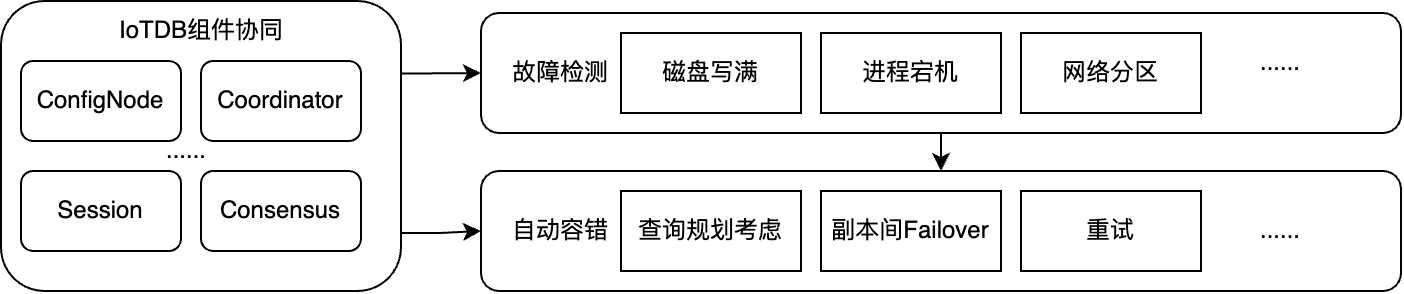
\includegraphics[width=0.99\linewidth]{1-overview-arch.png}
  \caption{IoTDB整体的高可用框架}
  \label{fig:c01-overview-arch}
\end{figure}

2. 将定义的高可用框架付诸实践,提高系统的故障检测和自动恢复能力。通过更加全面的故障检测,IoTDB能够更早、更准确地发现集群中发生的各种故障。在系统检测到故障之后,无需人工干预即可自动执行故障转移、节点替换、数据修复等操作,提升IoTDB分布式系统的韧性,使其能够应对更广泛的故障场景,减少人工干预的需求,并缩短故障恢复时间,从而保障系统的持续可用性,如图\ref{fig:c01-overview-arch}所示。

3. 对高可用架构和实现进行进行全面的测试与验证。本文将设计一系列覆盖各种故障场景的测试用例,包括模拟节点失效、网络分区、磁盘故障等。测试将关注系统的故障检测速度、恢复时间、数据一致性、以及对系统整体性能的影响等方面。通过严谨的实验和数据分析,我们将验证所构建的高可用性架构是否能够达到预期的目标。



\section{主要贡献}

本文的贡献主要体现在以下几个方面:

1. 提出了针对分布式系统故障场景和高可用架构的整体建模方法。本文研究了分布式系统中常见的故障种类,分析了故障的共性,并在此基础上提出了IoTDB高可用的整体方法论和架构。


2. 实现了高可用整体架构中的关键故障检测能力和自动容错和恢复能力。本文构建了更加完善的故障检测机制,并针对所有的故障建设自动容错能力,通过ConfigNode、客户端Session、服务端协调者、服务端共识模块等多个关键组件的协同,使得集群能够有效应对更广泛的故障类型,提升系统的韧性。


3. 进行了大量的测试和实验,证明了该高可用架构能够有效解决现有问题并应对新的挑战,为构建高可靠的分布式系统提供了实践支撑和数据验证。


\section{组织结构}
本文共分为8个章节,每个章节的内容如下:

第1章为引言部分,介绍了工业物联网、时间序列数据、时序数据库、Apache IoTDB、分布式数据库中的高可用性和容错能力等背景,阐述了本文建设更极致、更完善的可用性的研究动机,概括了本文的研究内容和研究贡献,描述了本文的组织结构。

第2章为相关研究综述,重点介绍了学术界对于分布式系统故障、高可用容错相关的研究,以及工业界多个广泛应用的分布式系统中的高可用方案的介绍。

第3章介绍了集群的故障检测和发现机制,包括基于ConfigNode Leader和DataNode之间心跳的节点存活探测、基于DataNode和DataNode之间心跳的集群拓扑探测、基于Phi Accrual算法的故障研判机制、基于集群监控的故障发现能力,和加速故障发现的若干优化。

第4章介绍了集群的故障恢复和容错能力,包括客户端、协调者、共识模块的三层联合容错机制。介绍了共识模块提供的数据副本容错基础,协调者模块利用多副本重试的容错尝试,客户端利用重试解决集群的暂时故障状态或不一致状态的能力,并阐述了故障时期的熔断和降级措施。

第5章介绍了集群对于经典故障场景的容错流程。结合第3章的故障检测和发现机制、第4章的故障恢复和容错机制,IoTDB集群能够抵御例如磁盘写满、进程宕机、网络对称/非对称分区、集群变更时的不一致等问题,并给出每种场景的详细容错流程。

第6章为实验部分。

第7章介绍了本文的工作总结和不足之处,并指出了未来工作的主要方向。